\chapter{Data}

\section{Datasets}

\subsection{Lyrics dataset}
 We chose the \textit{55000+ Song Lyrics dataset} from Kaggle.com\todo{tady by se hodila footnote s linkem na dataset} to obtain lyrics data. The Kaggle dataset originally contained 57 650 English songs. It’s lyrics are scraped from LyricsFreak. Extremely long and short lyrics were removed as well as all non-ASCII symbols from the lyrics. This is the dataset we used to train our text-based recommendation methods. Figure \ref{fig:lyrics_dataset} shows the first two entries of the dataset.\\
 \begin{figure}[h]
    \centering
	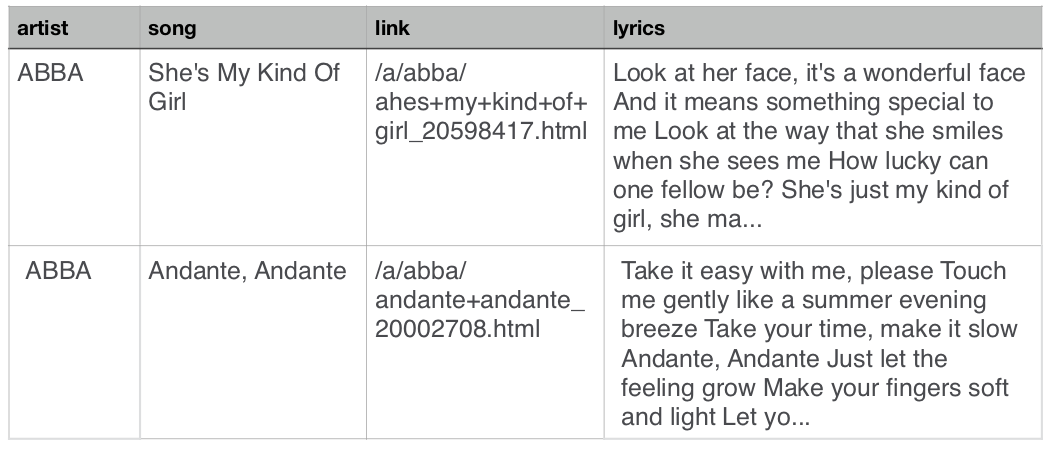
\includegraphics[height=60mm]{./img/dataset_preview.png}
	\caption{First two entries of the 55000+ Lyrics Dataset}
	\label{fig:lyrics_dataset}
\end{figure}

\subsection{User-information dataset}
To evaluate text and audio based methods on real-life user data, we had to select a dataset containing song information and lyrics as well as a dataset with information about users and their played tracks. First we tried to match the lyrics dataset onto the \textit{Echo Nest Taste Profile subset} \todo{stejne jako u predchozich datasetu, pridej footnote s linkem} from the Million Song Dataset website. However we only had 6800 songs with lyrics as well as user data.  We then tried the \textit{Thisismyjam} dataset also available on MSD. After removing songs we did not have lyrics for, we ended up with 16594 unique songs, and 45054 unique users. For each of the 16594 songs we also acquired a mono .wav file. \todo[inline]{Tady nevim, jestli mam rikat, ze jsem to stahla z YouTube, jestli je to jako v pohode. LP: asi bych to nechal takto - myslim ze detaily tady nejsou nezbytne a potencialne by to mohlo byt problematicke...}. \\
\todo[inline]{Myslim ze by se hodilo pridat nejake informace o tom thisismyjam datasetu - jake typy dat obsahuje, jak byly ziskane, info o tom, ze uzivatele sestavuji playlisty nebo tak neco - celkove je kapitola 2 mozna az prilis stroha...}

\section{Final dataset statistics}
Overall our final dataset had 160454 entries containing a user id, the artist, the song title and the lyrics. As our evaluation method is based on the users playlists (we took a portion of their played songs and tried to calculate the missing ones based on our metrics\todo{Co treba: aimed to reveal the missing entries based on the implemented recommending techniques} - will be described in more detail in the \textit{Experiment section}) we studied the dataset and especially the playlist length in more detail.\\
Here are some important remarks:
\begin{itemize}
    \item Each user only has one playlist.
    \item We do not know, how many times a user played a song.
    \item We do not know which songs the user has played most recently.
    \item Users with only one song are useless for our evaluation.
    \item It should be easier to complete the dataset for users with longer datasets.
\end{itemize} 
When analyzing our dataset, it turned out, that out of 45054 users or lets say playlists\todo{to users vs. playlists by chtelo presne definovat v predchozi sekci a pak pouzivat konzistentne ve zbytku prace.}, there are 22257 with only one song, which leaves us with 22797 we can use. Meaning, more than half of the playlists (about 51\% is useful for our evaluation as shown in figure \ref{fig:useless_users}.

The distribution of useful playlist lengths is shown in more detail in Figure \ref{fig:playlist_lenght_distribution}. We can see that most of the playlists are short, almost a third of them only contains two songs. The average number of songs per playlists (including those containing only one song) is 3.56. 
\begin{figure}[ht]
    \centering
	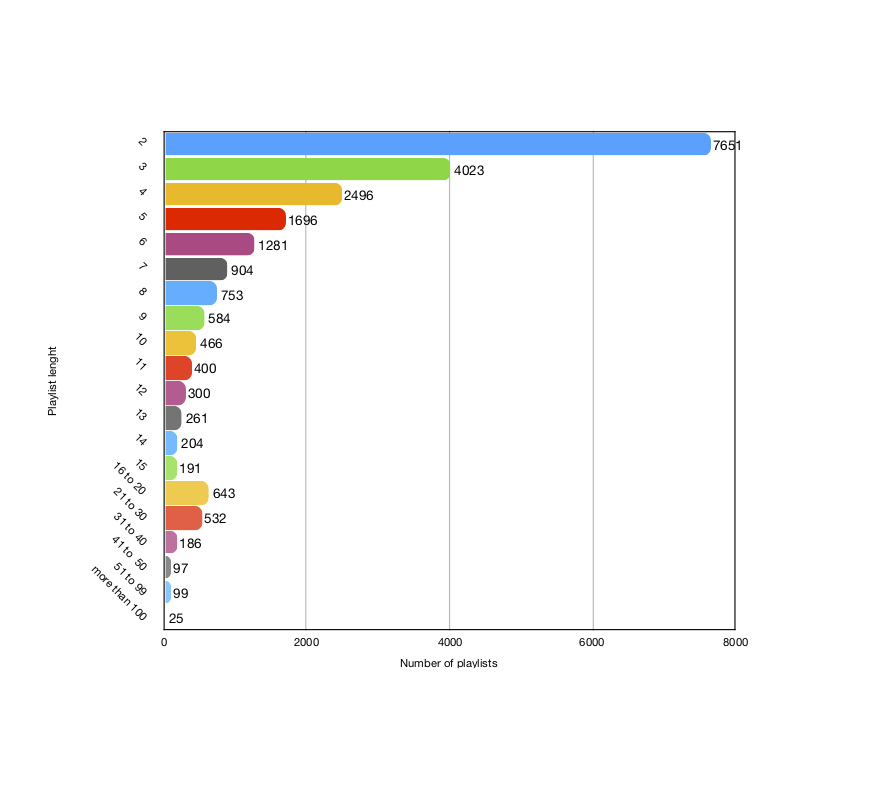
\includegraphics[height=110mm]{./img/playlist_description.png}
	\caption{The number of playlists for different lenghts}
	\label{fig:playlist_lenght_distribution}
\end{figure}
\todo[inline]{Tady mi to o 5 pisnicek nevychazi, takze to budu muset prepocitat, spis co rikate na tenhle graf? Pripadne jeste neco byste sem dodal? LP: graf vypada dobre}

Each song\todo{Kazda asi ne:-) informace je jasna, ale chce to preformulovat...} has been played by 10.84 users on average. The distribution and the most popular songs are depicted in Figure \ref{fig:popular_song_distribution}. The by far most popular song with a total of 816 plays was \textit{Royals} by \textit{Lorde}. Second came \textit{Radioactive} by \textit{Imagine Dragons} with 674 users who played it. All other songs have been played by less than 500 users.

\begin{figure}[ht]
    \centering
	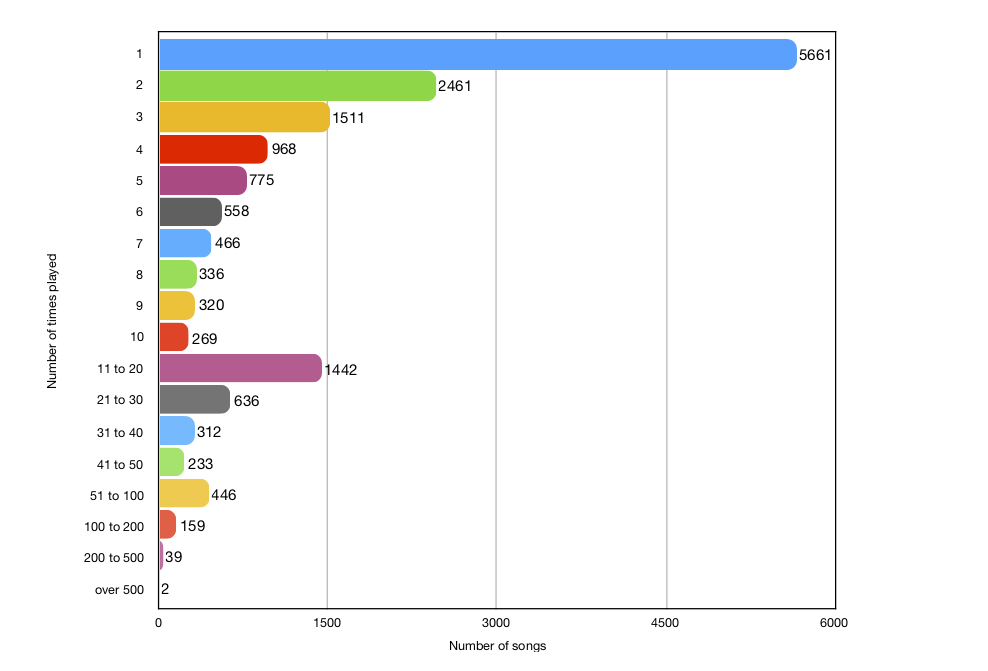
\includegraphics[height=80mm]{./img/popular_song_distribution.png}
	\caption{The number of playlists a song was in}
	\label{fig:popular_song_distribution}
\end{figure}\todo{U figure 2.3 je nepresny popisek osy Y}
